%	file:		thesis.tex
%	author:	alex c. williams
%	updated:	6 May 2015

%	description:
%	this file provides a template for the mtsu computer science thesis.
%
%	NOTES
%	1. Chapter Headings should be bold in the "text" portion of the document.
%	- To fix:
%		1. add /textbf to each /chapter{} line
%		2. compile
%		3. remove \textnormal from the \thesection renew command.
%		4. compile
%
%	2. To change "Professor One" and etc., you need to modify the names in the complementary "committee_header.tex" file.

\documentclass[12pt, oneside]{book}

% Include these packages:
\usepackage[top=3.17cm, bottom=2.54cm, left=3.81cm, right=2.54cm]{geometry}	 % for margin requirements.
\usepackage{mathptmx}% http://ctan.org/pkg/mathptmx
\usepackage{setspace} % for double-spacing.
\usepackage{xifthen}%
\doublespacing
\usepackage{lipsum}
\usepackage{tocloft}
\usepackage{color}
\usepackage{array}
\usepackage{stfloats}
\usepackage[pdftex]{graphicx}
\usepackage{subcaption}
\usepackage[export]{adjustbox}
\usepackage{multirow}
\usepackage{url}
\usepackage{changepage}
\usepackage{floatrow}
\usepackage{titlesec}
\usepackage{fancyhdr}
\usepackage{chngcntr}
\usepackage{fancyhdr}

% -- Define code snippet configuration
\usepackage{listings}
\usepackage{color}

%MULTIROWS
\usepackage{multirow}
\usepackage{amssymb}

\definecolor{dkgreen}{rgb}{0,0.6,0}
\definecolor{gray}{rgb}{0.5,0.5,0.5}
\definecolor{mauve}{rgb}{0.58,0,0.82}

\lstset{frame=tb,
  language=Java,
  aboveskip=3mm,
  belowskip=3mm,
  showstringspaces=false,
  columns=flexible,
  basicstyle={\small\ttfamily},
  numbers=none,
  numberstyle=\tiny\color{gray},
  keywordstyle=\color{blue},
  commentstyle=\color{dkgreen},
  stringstyle=\color{mauve},
  breaklines=true,
  breakatwhitespace=true,
  tabsize=3
}

% -- Base Page Styling 
\floatsetup[table]{capposition=top}
\counterwithout{figure}{chapter}
\counterwithout{table}{chapter}
\setlength\textfloatsep{18mm}
\fancyhf{}
\fancyhead[R]{\thepage}

% -- Base Styling for Section/Subsection/Subsubsection --
\titlespacing{\section}{0pt}{\parskip}{-\parskip}
\titlespacing{\subsection}{0pt}{\parskip}{-\parskip}
\titlespacing{\subsubsection}{0pt}{\parskip}{-\parskip}

% Styling for Section Headers
\titleformat{\section}
{\normalfont\bfseries\filcenter}
{\textnormal\thesection}
{0cm}
{}

% Styling for Subsection Headers
\titleformat{\subsection}
{\normalfont\filcenter}
{\textnormal\thesubsection}
{0cm}
{}

% -- Stylize Subfigure Headings--
\newlength\Origarrayrulewidth
\renewcommand{\thesubfigure}{\Alph{subfigure}}
\newcommand{\Cline}[1]{%
 \noalign{\global\setlength\Origarrayrulewidth{\arrayrulewidth}}%
 \noalign{\global\setlength\arrayrulewidth{2pt}}\cline{#1}%
 \noalign{\global\setlength\arrayrulewidth{\Origarrayrulewidth}}%
}
\newcommand\Thickvrule[1]{%
  \multicolumn{1}{!{\vrule width 2pt}c!{\vrule width 2pt}}{#1}%
}

% -- Stylize the Table of Contents --
\renewcommand{\cfttoctitlefont}{\hfill\normalsize}
\renewcommand*\thesubsection{}
\renewcommand*\thesection{\textnormal}
\renewcommand*\thechapter{\Roman{chapter}.}
\renewcommand*\thepart{}
\renewcommand\cftchapfont{\mdseries}
\renewcommand{\cftchapleader}{\cftdotfill{\cftdotsep}}
\renewcommand\cftchappagefont{\normalfont}
\renewcommand\cftpartpagefont{\normalfont}
\renewcommand\contentsname{\hfill{\textbf{TABLE OF CONTENTS}}\hfill}
\renewcommand{\cftaftertoctitle}{\hfill}
\renewcommand{\cftbeforepartskip}{1.00em}

% -- Stylize Chapter Headings --
\makeatletter
\let\orig@chapter\@chapter
\def\@chapter[#1]#2{\ifnum \c@secnumdepth >\m@ne
                       \if@mainmatter
                         \refstepcounter{chapter}%
                         \typeout{\@chapapp\space\thechapter.}%
                         \addcontentsline{toc}{chapter}%
                                   {\textnormal{CHAPTER}~\protect\numberline{\thechapter}#1}%
                       \else
                         \addcontentsline{toc}{chapter}{#1}%
                       \fi
                    \else
                      \addcontentsline{toc}{chapter}{#1}%
                    \fi
                    \chaptermark{#1}%
                    \addtocontents{lof}{\protect\addvspace{10\p@}}%
                    \addtocontents{lot}{\protect\addvspace{10\p@}}%
                    \if@twocolumn
                      \@topnewpage[\@makechapterhead{#2}]%
                    \else
                      \@makechapterhead{#2}%
                      \@afterheading
                    \fi}
\makeatother

% Stylize List of Figures
\renewcommand*\listfigurename{LIST OF FIGURES}
\renewcommand{\cftloftitlefont}{\hfill\normalsize}
\renewcommand{\cftafterloftitle}{\hfill}
\setlength{\cftbeforeloftitleskip}{-3em}
\setlength{\cftafterloftitleskip}{-0.05em}
\renewcommand{\cftfigfont}{Figure }


\usepackage{titlesec}
\usepackage[tracking=true]{microtype}
\titleformat{\chapter}[display]
  {\vspace{-2.54cm}\normalsize}
  {\filcenter\textbf{\MakeUppercase{\chaptertitlename} \thechapter}}
  {\parskip}
  {\filcenter\thispagestyle{myheadings}}

\titlespacing{\chapter}{0pt}{50pt}{\parskip}

\fancyhead[L]{}

% Stylize List of Tables
\renewcommand*\listtablename{LIST OF TABLES}
\renewcommand{\cftlottitlefont}{\hfill\normalsize}
\renewcommand{\cftafterlottitle}{\hfill}
\setlength{\cftbeforelottitleskip}{-3em}
\setlength{\cftafterlottitleskip}{-0.05em}
\renewcommand{\cfttabfont}{Table }
\renewcommand{\cftfigaftersnum}{ -- }
\renewcommand{\cfttabaftersnum}{ -- }

\renewcommand{\thefigure}{\arabic{figure}}
\renewcommand{\thetable}{\arabic{table}}
\renewcommand{\theequation}{}

% -- Stylize Equations --
\makeatletter
\def\@eqnnum{{\normalfont \normalcolor \theequation}}
\makeatother

% -- Stylize Bibliography Title --
\renewcommand{\bibname}{\textbf{BIBLIOGRAPHY}}

% Include the dependency
% command for 
\newenvironment{nscenter}
 {\parskip=0pt\par\nopagebreak\centering}
 {\par\noindent\ignorespacesafterend}

% Change margins on-command.
\def\changemargin#1{\list{}{\leftmargin#1}\item[]}
\let\endchangemargin=\endlist 

% Macro:	addTitleAndAuthor
% Parameters:
%	- 1: Title Name
%	- 2: Your Name
\newcommand{\addTitleAndAuthor}[2]{
\begin{nscenter} 
\mbox{ }\\
  % Process Title..
#1% if #1 is not empty
\\[\baselineskip]

By\\[0\baselineskip]

#2
\\[2\baselineskip]% if #1 is not empty

\end{nscenter}
}

\newcommand{\addCommitteeMember}[2][Computer Science]{
	\ifthenelse{\isempty{#1}}
	{\\[0\baselineskip] \underline{\hspace{11.54cm}} \\[0\baselineskip] Dr. professor's name (Computer Science or other department)\\[0\baselineskip]}
	{\\[0\baselineskip] \underline{\hspace{11.54cm}} \\[0\baselineskip] Dr. {#2} (#1) \\[0\baselineskip]}
}


\newcommand{\addSupervisor}[2][Computer Science]{
	\ifthenelse{\isempty{#1}}
	{\\[0\baselineskip] \underline{\hspace{11.54cm}} \\[0\baselineskip] Supervisor Dr. professor's name (Computer Science) \\[0\baselineskip]}
	{\\[0\baselineskip] \underline{\hspace{11.54cm}} \\[0\baselineskip] Supervisor Dr. {#2} (#1) \\[0\baselineskip]}
}

\newcommand{\addChair}[1][Chair's Name]{
	\noindent\underline{\hspace{11.54cm}} \newline Dr. #1, Chairperson Computer Science Department \\
}

\newcommand{\addDean}[1][Dean's Name]{
	\noindent\underline{\hspace{11.54cm}} \newline Dr. #1, Interim Dean of the College of Graduate Studies
}

% Macro:	addCommittee
% Parameters:
%	- 1. Committee Member 1 (Supervisor)
%	- 2. Committee Member 1's Department
%	- 3. Committee Member 2
%	- 4. Committee Member 2's Department
%	- 5. Committee Member 3
%	- 6. Committee Member 3's Department
%	- 7. Computer Science Chairperson
%	- 8. Dean of Graduate Studies
\newcommand{\addCommittee}[8]{
	\noindent APPROVED: 
	\begin{changemargin}{2.54cm}
		Graduate Committee\vspace{1mm} \newline
		% set committee members
		\addSupervisor[#2]{#1}
		\addCommitteeMember[#4]{#3}
		\addCommitteeMember[#6]{#5}
	\end{changemargin}

	\addChair[#7]

	\addDean[#8]

}

\newcommand{\addDegreeNotes}[1]{
\vspace{8ex}
\centerline{A qualifying paper submitted in partial fulfillment}
\centerline{of the requirements for the degree of}

\vspace{8ex}

\centerline{DOCTOR OF PHILOSOPHY}
\centerline{in}
\centerline{Computational Science}

\vspace{8ex}

\centerline{Middle Tennessee State University}
\vspace{1ex}

\centerline{#1}

\vspace{8ex}

\centerline{Project Supervisor:}

\centerline{Dr. Hong}

}

\usepackage{fancyheadings}

% Document Formation
\begin{document}
% - - - Title Page - - - 
% Add Title / Author
%\thispagestyle{empty}

%\addTitleAndAuthor	{\textbf{COMPUTATIONALLY ACCELERATED PAPYROLOGY}} % Title
%				{Alex C. Williams} % Author

% Add Committee
%\addCommittee{Hyrum D. Carroll}{Computer Science}
%			{John F. Wallin}{Physics and Astronomy}
%			{Cen Li}{Computer Science}
%			{Chrisila Pettey}
%			{Jackie Eller}

%\newpage
% - - - Title Page (with MS/Graduation Date)
% Add Title / Author
\pagenumbering{roman}
\thispagestyle{empty}
\pagestyle{fancy}
\lhead{} \chead{} \rhead{}
\lfoot{} \cfoot{\thepage} \rfoot{}
\renewcommand{\headrulewidth}{0pt}
\renewcommand{\footrulewidth}{0pt}
\vspace{2ex}
\addTitleAndAuthor	{\textbf{REM SLEEP STAGE IDENTIFICATION WITH WAVELET DECOMPOSITION AND ARTIFICIAL NEURAL NETWORK USING A SINGLE CHANNEL EEG}} % Title
				{Gabriel Toban} % Author

% Specify Graduate Month
\addDegreeNotes{May 2020}

\newpage
% - - - Acknowedglements Page - - -
\centerline{\textbf{ACKNOWLEDGEMENTS}}

This paper would not have been possible without the assistance of many people that I owe many thanks. Shuzhe Xu explained wavelet coefficients, coded the wavelet decomposition in MATLAB, and provided sound advice throughout the project. William H. Noah MD and Moataz Toban MD explained sleep staging and sleep medicine in general. Todd Gary PhD provided advice and connected me with so many opportunities. Don Hong PhD steered the direction of this paper with a seemingly infinite depth of knowledge. John Wallin PhD is the reason this paper is possible. There are many more who are not directly mentioned. Thank you all.

\newpage
\centerline{\textbf{ABSTRACT}}

The abstract can be no more than 150 words.  It goes on this page.

%\newpage
%\centerline{\textbf{PREFACE}}
%If you require a preface, type it here.

% - - - Table of Contents - - -
\newpage
\begingroup
\renewcommand{\vspace}[2]{}% Gobble 2 arguments after \vspace
\tableofcontents
\endgroup

\cleardoublepage
\clearpage

% - - - List of Tables - - -
\renewcommand\listtablename{\textnormal{LIST OF TABLES}}
\addcontentsline{toc}{chapter}{\listtablename}
\listoftables
\thispagestyle{plain}
\clearpage

% - - - List of Figures - - -
\renewcommand\listfigurename{\textnormal{LIST OF FIGURES}}
\addcontentsline{toc}{chapter}{\listfigurename}
\listoffigures
\clearpage

\newpage
\pagenumbering{arabic} % -- Change the page numbering and style.
\pagestyle{fancy}
\lhead{} \chead{} \rhead{\normalsize\thepage} % -- Change location of page number.
\lfoot{} \cfoot{} \rfoot{}
\renewcommand{\headrulewidth}{0pt}
\renewcommand{\footrulewidth}{0pt}

\chapter{\textbf{INTRODUCTION}}
Sleep stages are the most precise way to separate wakefulness from sleep state. Physiologic and pathologic events can be identified and studied through examining stages of sleep or sleep stages. Certain health insurances require that wakefulness is separated from sleep state using an electroencephalogram (EEG) in order for a sleep study to be conducted. 

An EEG uses electrodes placed on the head to detect electric potentials in the brain. The difference between the electric potentials of two electrode positions, called an EEG channel or channel, are recorded in regular intervals to produce brain waves. One electrode is the active electrode while the other is the reference electrode \cite{berry_md_chair_aasm_nodate}. The electrode positions are well-defined by the International 10/20 system \cite{berry_md_chair_aasm_nodate} \cite{noauthor_10/20_nodate-1} \cite{noauthor_10/20_nodate}. The EEG channels that are best to use were standardized originally by Rechtscheffen and Kales \cite{rechtschaffen_manual_nodate} commonly known as the R\&K standard. The American Academy of Sleep Medicine (AASM) maintains and updates the R\&K standard today.

Sleep stages are typically identified with a combination of parameters known as a polysomnographic record (PSG). These parameters include, but are not limited to, electroencephalogram (EEG) derivations, electrooculogram (EOG) derivations, and a chin electromyogram (EMG) \cite{berry_md_chair_aasm_nodate}. Elements from all 3 are used to identify sleep stages \cite{berry_md_chair_aasm_nodate}. An EEG monitors brainwaves. An EOG monitors eye movements. An EMG monitors muscle movements. EEGs, EOGs, and EMGs all can use electrodes placed on the head and face. 

An alternative to a PSG is an at home study. There can be many electrodes and channels used in a PSG. The AASM recommends that 8 electrode positions creating 6 channels are used for an EEG alone \cite{berry_md_chair_aasm_nodate}. Using this many channels and the variety of parameters for the PSG requires special training to use, special training to interpret, expensive equipment, and likely a lab. Some at home studies use a single channel EEG requiring very little training to use, cheaper equipment, and no lab. The at home study still requires special training to interpret.

Automated sleep staging can be accomplished with a combination of parameters from a PSG \cite{sinha_artificial_2008} \cite{fraiwan_automated_2012} \cite{rao_detecting_2014} \cite{kurt_ann-based_2009} \cite{shambroom_validation_2012} or a single channel EEG \cite{ventouras_sleep_2005} \cite{ebrahimi_automatic_2008} \cite{crasto_wavelet_2017} \cite{alvarez_usefulness_2017}. Ebrahimi et al. achieved 93\% accuracy using the wavelet decomposition of a single channel EEG and a neural network \cite{ebrahimi_automatic_2008}. Kurt et al. achieved 97-98\% accuracy using the wavelet decomposition of EEG, EOG, and chin-EMG \cite{kurt_ann-based_2009}. 

In order to automate sleep staging with an at home study, wavelet decomposition of a single channel EEG was used identify REM sleep using a feed-forward back-propagation (FFBB) artificial neural network (ANN). Chapter 2 explores the factors of picking a single EEG channel, the reasons to use wavelet decomposition for signal processing, and the reasons behind the feed-forward back-propagation ANN. Chapter 3 explains the exact methods and results. Chapter 4 discusses the conclusions and future studies.
\chapter{\textbf{BACKGROUND}}

\section{\textbf{The Single Channel EEG}}
An EEG uses electrodes placed on the head to detect electric potentials in the brain. The difference between the electric potentials of two electrode positions, called an EEG channel or channel, are recorded in regular intervals to produce brain waves. The electrode positions are well-defined by the International 10/20 system \cite{berry_md_chair_aasm_nodate} \cite{noauthor_10/20_nodate-1} \cite{noauthor_10/20_nodate}. The EEG channels that are best to use were standardized originally by Rechtscheffen and Kales \cite{rechtschaffen_manual_nodate} commonly known as the R\&K standard. The American Academy of Sleep Medicine (AASM) maintains and updates the R\&K standard today.

Brain waves, activities, and events are defined by the amplitude, frequency, and identifying factors of a single wave or grouping of waves. There are 5 EEG frequencies defined in table \ref{tab:freq}. The identifying factors include things such as what happens before/after the wave, the difference in peeks of wave, and how much a wave stands out. \cite{berry_md_chair_aasm_nodate}. Waves, activities, or events, such as spindles or arousals, can be identified by a combination of these identifying factors, the frequency, and the amplitude \cite{berry_md_chair_aasm_nodate}. 

\begin{table}[H]
	{\hspace{0cm}
		\begin{tabular}{|p{5cm}|c|c|}
			\hline \\ [-1.5ex]
			\textbf{Name} & \textbf{Frequency (Hz)} & \textbf{Peak-to-Peak Amplitude (uV)} \\
			\hline \\ [-1.5ex]
			Slow Wave Activity & 0.5-2.0 & $>$75 \\
			\hline \\ [-1.5ex]
			Delta Waves & 0-3.99 & N/A \\
			\hline \\ [-1.5ex]
			Theta Waves & 4-7.99 & N/A \\
			\hline \\ [-1.5ex]
			Alpha Waves & 8-13 & N/A \\
			\hline \\ [-1.5ex]
			Beta Waves & $>$13 & N/A \\
			\hline
		\end{tabular}
	} 
\caption{The frequency and peak-to-peak amplitude of different brain waves as identified by the AASM \cite{berry_md_chair_aasm_nodate}.}
\label{tab:freq}
\end{table}

The international 10/20 system uses labels with letters and numbers to identify the different electrode positions on the head referenced in figure \ref{fig:1020}. The letters identify the brain lobe that the electrode is over identified in table \ref{tab:1020letters}. The numbers identify the position in the direction going from one ear to the other. To find each position, a technician begins at a starting position and moves around the head in percentages. \cite{noauthor_10/20_nodate} \cite{noauthor_10/20_nodate-1}


\begin{figure}[H]
	\centering
	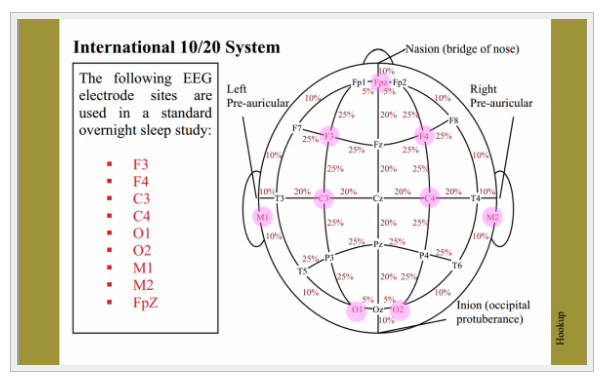
\includegraphics[]{1020.png}
	\caption{A representation of the electrode positions identified by the 10/20 system. It originated from https://sleeptechstudy.wordpress.com/category/1020-system/ \cite{noauthor_10/20_nodate}. Each position is labeled by 1 to 3 letters and/or a number which are listed on the left side of this image.}
	\label{fig:1020}
\end{figure}


\begin{table}[H]
	{\hspace{0cm}
		\begin{tabular}{|p{5cm}|c|}
			\hline \\ [-1.5ex]
			\textbf{Abbreviation} & \textbf{Brain Lobe/Region} \\
			\hline \\ [-1.5ex]
			Fp & Frontal pole \\
			\hline \\ [-1.5ex]
			F & Frontal  \\
			\hline \\ [-1.5ex]
			T & Temporal \\
			\hline \\ [-1.5ex]
			C & Central \\
			\hline \\ [-1.5ex]
			P & Parietal \\
			\hline \\ [-1.5ex]
			O & Occipital \\
			\hline \\ [-1.5ex]
			M & Mastoid \\
			\hline
		\end{tabular}
	} 
	\caption{The brain region that relates to every electrode location. It originated from https://sleeptechstudy.wordpress.com/category/1020-system/ \cite{noauthor_10/20_nodate}.}
	\label{tab:1020letters}
\end{table}

EEG channels are defined by two electrode positions. For an adult EEG, the AASM recommends the channels listed in table \ref{tab:AASMchrec}. The data used for this study does not use the channels recommended by the AASM \cite{noauthor_sleep-edf_nodate}, but the efficacy of the alternative electrode positions are described by van Sweden et al. \cite{b_alternative_1990}. 

\begin{table}[H]
	{\hspace{0cm}
		\begin{tabular}{|p{5cm}|c|}
			\hline \\ [-1.5ex]
			\textbf{Recommended} & \textbf{Acceptable} \\
			\hline \\ [-1.5ex]
			F4-M1 & Fz-Cz \\
			\hline \\ [-1.5ex]
			C3-M1 & Cz-Oz  \\
			\hline \\ [-1.5ex]
			O2-M1 & C4-M1\\
			\hline
		\end{tabular}
	} 
	\caption{The channels for an EEG to identify sleep stages as recommended by the AASM \cite{berry_md_chair_aasm_nodate}. Each electrode has backup electrode. Some important backups are Fpz for Fz and Cz for C3.}
	\label{tab:AASMchrec}
\end{table}

Different electrode positions and channels detect different brain waves, activities, and events. Table \ref{tab:wavetolobe} list some of the brain waves, activities, and events and which lobe position or channel detects them. This is one the reasons to use multiple channels for an EEG. 

\begin{table}[H]
	{\hspace{0cm}
		\begin{tabular}{|p{2cm}|c|c|c|c|c|c|}
			\hline \\ [-1.5ex]
			& \textbf{Slow Wave} & \textbf{V-Waves} & \textbf{K-complexes} & \textbf{Spindles} & \textbf{Sawtooth} & \textbf{Alpha} \\
			\hline \\ [-1.5ex]
				\textbf{Frontal} &  &  & Maximal &  &  &  \\
			\hline \\ [-1.5ex]
			\textbf{Central} &  & Maximal &  & Maximal & Maximal & Adequate \\
			\hline \\ [-1.5ex]
			\textbf{Occipital} &  &  &  &  &  & Maximal  \\
			\hline \\ [-1.5ex]
			\textbf{Fz-Cz} & No &  &  &  &  &\\
			\hline \\ [-1.5ex]
			\textbf{E1-Fpz} & Yes &  & & &  & \\
			\hline
		\end{tabular}
	} 
	\caption[The brain regions/electrode channel that brain waves, activities, and events (marker) are most likely to appear.]{The brain regions/electrode channel that brain waves, activities, and events (marker) are most likely to appear. To understand what stages are identified with each marker, reference the AASM scoring guide \cite{berry_md_chair_aasm_nodate}. Blanks space mean there was not any specifications for this region/channel and marker combination. The “Yes” means that this channel does identify Slow Waves while the “No” means that the channel does not identify Slow Waves. “Maximal” implies the maximal wave amplitude will be recognized. “Adequate” means adequate for identification. All the information except “Adequate” was gathered from the AASM scoring guide \cite{berry_md_chair_aasm_nodate}. The “Adequate” comes from the R\&K standard \cite{rechtschaffen_manual_nodate}. E1-Fpz is the frontal regions referenced to the contralateral ear or mastoid.}
	\label{tab:wavetolobe}
\end{table}

The definition and number of sleep stages has evolved over time. The R\&K standard originally defined 7 stages to identify sleep excluding non rapid eye movement (NREM) which is a combination of stage 1, 2, 3, and 4 \cite{rechtschaffen_manual_nodate}. The AASM defines 5 stages to identify sleep \cite{berry_md_chair_aasm_nodate}. The AASM definition excludes Movement Time and combines stage 3 and 4. Table \ref{tab:stage} list all the stages from R\&K. The data used for this study follows the R\&K standard stages with an extra identifier for unknown or ungraded stages \cite{noauthor_sleep-edf_nodate}.

\begin{table}[H]
	{\hspace{0cm}
		\begin{tabular}{|c|c|}
			\hline \\ [-1.5ex]
			\textbf{R\&K} & \textbf{AASM} \\
			\hline \\ [-1.5ex]
			Wakefulness (W) &	Wakefulness (W) \\
			\hline \\ [-1.5ex]
			Movement Time (MT) & \\
			\hline \\ [-1.5ex]	 
			Stage 1	& NREM 1 (N1) \\
			\hline \\ [-1.5ex]
			Stage 2	& NREM 2 (N2) \\
			\hline \\ [-1.5ex]
			Stage 3 & \multirow{2}{*}{NREM 3 (N3)}\\
			\cline{1-1} \\ [-1.5ex]
			Stage 4 & \\
			\hline \\ [-1.5ex]
			NREM (1,2,3,4)	& \\
			\hline \\ [-1.5ex] 
			REM (R) & REM (R)  \\
			\hline
		\end{tabular}
	} 
	\caption[The different sleep stages as identified by the R\&K \cite{rechtschaffen_manual_nodate} and the AASM \cite{berry_md_chair_aasm_nodate}.]{The different sleep stages as identified by the R\&K \cite{rechtschaffen_manual_nodate} and the AASM \cite{berry_md_chair_aasm_nodate}. It is important to note that Movement Time (MT) and Non-REM (NREM) are still used. Also, NREM 3 from the AASM is a combination of Stage 3 and Stage 4 from R\&K.}
	\label{tab:stage}
\end{table}

Different brain waves, activities, and events (EEG markers) help define different sleep stages. Every sleep stage is completely defined according to the AASM using many factors of a PSG (polysomnogram) including the EEG, EOG, and EMG \cite{berry_md_chair_aasm_nodate}. For example, REM stage sleep uses an EOG to identify the rapid eye movement the stage is named after, but it may be identified with sawtooth waves detected by an EEG. Automated sleep staging with an EEG does not consider all the additional defining parameters from the PSG. Table \ref{tab:stagetoWave} gives an idea of the relationship between EEG markers and sleep stages. 

\begin{table}[H]
	{\hspace{0cm}
		\begin{tabular}{|p{3cm}|c|c|c|c|c|}
			\hline \\ [-1.5ex]
			& \textbf{W} & \textbf{N1} & \textbf{N2} & \textbf{N3} & \textbf{REM} \\
			\hline \\ [-1.5ex]
			\textbf{Slow Wave} &  &  &  & R &\\
			\hline \\ [-1.5ex]
			\textbf{V-Waves}  &  & NR &  &  &\\
			\hline \\ [-1.5ex]	 
			\textbf{K-complexes} &  & P & R &  & P\\
			\hline \\ [-1.5ex]
			\textbf{Spindles} &  & P & R &  & P\\
			\hline \\ [-1.5ex]
			\textbf{Sawtooth}&  &  &  &  & NR\\
			\hline \\ [-1.5ex]
			\textbf{Alpha}& NR & P &  &  & P\\
			\hline \\ [-1.5ex]
		    \textbf{Beta} & NR &  &  &  &\\
			\hline \\ [-1.5ex] 
			\textbf{LAMF \{theta\}} &  & R & P &  &  R\\
			\hline \\ [-1.5ex]
			\textbf{Theta} &  & P &  &  & \\
			\hline \\ [-1.5ex]	
			\textbf{No Arousal} &  &  & R &  & P \\
			\hline
		\end{tabular}
	} 
	\caption[Which sleep stages are identified by certain EEG markers as recommended by the AASM \cite{berry_md_chair_aasm_nodate}.]{Which sleep stages are identified by certain EEG markers as recommended by the AASM \cite{berry_md_chair_aasm_nodate}. It does not identify every possible marker. For example, stage N1 can follow stage W, stage N2, and stage R under different conditions. An arousal is the cause of many significant events including k-complexes. \\
	NR: Not Required; R: Required; P: Possible; \{Blank\}: Not mentioned or not possible}
	\label{tab:stagetoWave}
\end{table}
There is a current push to diagnose sleep associated diseases with a cheaper at home study. PSG requires expensive equipment and a technician present. The AASM \cite{berry_md_chair_aasm_nodate} recommends that at least 3 EEG channels, 2 EOG channels, and a chin EMG among other things for a PSG. Ventouras et al. \cite{ventouras_sleep_2005}, Ebrahimi et al. \cite{ebrahimi_automatic_2008}, and Crasto et al. \cite{crasto_wavelet_2017} all used a single EEG channel with accuracies between 85\% and 95\%. Shambroom et al. \cite{shambroom_validation_2012} tested current equipment that uses a single channel EEG to do sleep staging. Sleep staging using a single EEG channel would be cheaper than a PSG. This study will use a single EEG channel.

Aside from slow waves, any single brain wave, activity, or event (EEG marker) from an EEG is not uniquely required in only 1 sleep stage. Slow waves are identified by E1-Fpz channel, table \ref{tab:wavetolobe}, and identify stage N3, table \ref{tab:stagetoWave}. Although, Crasto et al. \cite{crasto_wavelet_2017} was able to break down stage N3 into stage 3 and 4 using channel Fpz-Cz. The dataset used in this study has channels Fpz-Cz and Pz-Oz available. The channel to identify slow waves is not available. Since all other waves in table \ref{tab:wavetolobe} are adequately identified in the central and frontal lobes, Fpz-Cz channel was used to for this study. Future studies may consider using other frontal lobe channels.

The AASM  and R\&K recommend that sleep staging is completed in 30 second epochs \cite{berry_md_chair_aasm_nodate} \cite{rechtschaffen_manual_nodate}. Each epoch is assigned a single sleep stage \cite{rechtschaffen_manual_nodate} \cite{berry_md_chair_aasm_nodate}. If an epoch exhibits features of more than one stage, the R\&K standard \cite{rechtschaffen_manual_nodate} strictly assigns each epoch the stage that takes the most of the epoch . The AASM \cite{berry_md_chair_aasm_nodate} has additional rules when the features of more than one stage are exhibited in any epoch. The R\&K standard \cite{rechtschaffen_manual_nodate} states 3 reason for 30 second epochs: too small epoch will be too cumbersome, too large epochs will miss out on epoch details, and paper sizes for EEG machines typically fit 30 seconds of data. The Physionet data set \cite{noauthor_sleep-edf_nodate} used in this study has 30 second epochs marked with their sleep stage. Current study uses 30 second epochs. The AASM and R\&K both mention the necessity to consider the stage before and after the epoch currently being scored. This study will use 3 epochs to stage a single epoch. In future studies, it may be best to identify each individual wave. Once each wave is identified, epochs will not be required. Each stage could be uniquely identified rather than being a potential group of stages identified by 1 stage.

REM sleep has not been the specific goal of any study found. REM sleep is the only stage that can be easily found by rapid eye movements. Rapid eye movements are not detected with an EEG. There is not a required unique identifier for REM sleep in the EEG. REM sleep is almost indistinguishable from N1 sleep in an EEG. Stages W, N1, N2, and N3 are easily distinguishable from each other with an EEG (see table \ref{tab:stagetoWave}). Stages N1, N2, and N3 all have a unique EEG marker to identify them. Current study will concentrate on REM sleep.  


\section{\textbf{Signal Processing and Wavelet Decomposition}}
A brainwave or a single channel from an EEG is a signal. It is a record of the difference in electrode potentials over time. Byrne \cite{byrne_signal_2014} states that the Fourier series is the most important tool in signal processing. Achermann \cite{achermann_eeg_2009} stated that Dietsch \cite{dietsch_fourier-analyse_1932} performed the first Fourier analysis on an EEG in 1932. 

The Fourier series of a function is \cite{debnath_wavelet_2014}

\begin{equation}
f(x)=\sum_{n=-\infty}^{\infty}c_n e^{- \frac{in\pi x}{l}}
\end{equation}
where 
\begin{equation}
c_n = \frac{1}{2l} \int_{-l}^{l} f(t) e^{- \frac{in\pi x}{l}}.
\end{equation}
The Fourier integral theorem takes the limit as l approaches infinite of the Fourier series. \cite{debnath_wavelet_2014}
\begin{equation}
f(x) = \frac{1}{2\pi} \int_{-\infty}^{\infty} e^{iwx}dw \int_{-\infty}^{\infty} e^{-iwt}f(t)dt
\end{equation}
The Fourier transform of a signal is derived from the Fourier integral \cite{debnath_wavelet_2014}.
\begin{equation}
F{f(t)} = \hat{f}(w) = \int_{-\infty}^{\infty} e^{-iwt}f(t)dt = \langle f,e^{iwt}\rangle
\end{equation}

All of these represent harmonic or sinusoidal waves. The transform and series go on forever. The frequency of the waves of a Fourier Transform represent the Spectral Density of the original wave \cite{noauthor_time-frequency_nodate}. The spectral density is a representation of the amplitude of a wave\cite{noauthor_spectral_2017}, but the sinusoidal component of the transform does not allow if to capture local information \cite{debnath_wavelet_2014}. In other words, abrupt changes in amplitude may not be captured. It is well-known that Fourier Transforms cannot investigate time and frequency simultaneously \cite{sinha_artificial_2008} \cite{ebrahimi_automatic_2008} \cite{kurt_ann-based_2009} \cite{crasto_wavelet_2017} \cite{debnath_wavelet_2014}.

Some of the different brain waves, activities, and events in the EEG signal are defined by abrupt changes in amplitude over time. V-Waves are defined as "sharply contoured waves with a duration less than 0.5 seconds" \cite{berry_md_chair_aasm_nodate} and literally look like a "V". K-complexes are defined by "a well-delineated, negative, sharp wave immediately followed by a positive component standing out from the background EEG, with total duration greater or equal to 0.5 seconds" \cite{berry_md_chair_aasm_nodate}. Figure \ref{fig:kandv} shows the V-Wave and K-complex.


\begin{figure}[H]
	\centering
	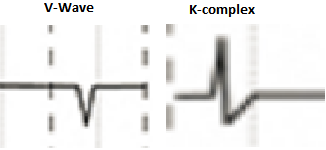
\includegraphics[]{VandK.png}
	\caption{The V wave and K-complex used in the sleep stage scoring manual from the AASM \cite{berry_md_chair_aasm_nodate}.}
	\label{fig:kandv}
\end{figure}

In order to provide descriptions of abrupt changes in amplitude over time like those found in the EEG signal, time-frequency signal analysis representations were created. Time-frequency representations can be classified as linear, quadratic, or higher-order representations. Hlawatsch and Boudreaux-Bartels listed at least 25 different time-frequency representations including 3 linear representations, Gabor, Short-time Fourier transform (STFT), and Wavelet transform (WT), and 2 quadratic representations, Choi-Williams Distribution (CWD) and Wigner Distribution (WD) \cite{hlawatsch_linear_1992}. Several of the other representations were modifications of WD \cite{hlawatsch_linear_1992}. The Wigner Distribution (WD), also known as Wigner-Ville Distribution (WVD), and the Choi-Williams Distribution are both generated from the Cohen "general class of bilinear shift-invariant, quadratic time-frequency distributions" \cite{debnath_wavelet_2014}. The WVD has been modified many times to create many time-frequency distributions \cite{debnath_wavelet_2014} \cite{noauthor_time-frequency_nodate}.

A general review of the methods used shows that Fourier and Wavelets are the primary representations used for analyzing an EEG in sleep staging \cite{alvarez_usefulness_2017}. Among those that used Fourier and Wavelets, the Wavelet representations resulted in the highest accuracies \cite{sinha_artificial_2008} \cite{ebrahimi_automatic_2008} \cite{kurt_ann-based_2009} \cite{crasto_wavelet_2017} \cite{alvarez_usefulness_2017}. Fraiwan et al. \cite{fraiwan_automated_2012} used Choi-Williams Distribution (CWD), continuous wavelet transform (CWT), and Hilbert-Huang Transform (HHT). Fraiwan et al. \cite{fraiwan_automated_2012} found that CWT had the highest accuracy. A Discrete Wavelet Transform (DWT) can decrease the processing time of a CWT \cite{debnath_wavelet_2014}. Ebrahimi et al. \cite{ebrahimi_automatic_2008} and Crasto and Upadhyay \cite{crasto_wavelet_2017} used Daubechies wavelet order 2 filter with DWT. Crasto and Upadhyay \cite{crasto_wavelet_2017} tested DWTs with Daubechies wavelet order 2 to 6 to decompose a signal for input into an artificial neural network (ANN) finding Daubechies wavelet order 2 to produce the most accurate results.

There are many time-frequency signal analysis representations that could be tested. The Gabor Transform, Short-time Fourier Transform, the Wigner Distributions, and many more could be tested with future studies. Since the Discrete Wavelet Transform has been tested with the highest accuracy, this study used DWT to decompose the signal. 

The discrete wavelet transform is based on the concept of a function called the "mother wavelet" \cite{debnath_wavelet_2014}.
\begin{equation}
\Psi_{a,b}(t) = \frac{1}{ \sqrt{|a|}} \Psi( \frac{t-b}{a}),\; a,b \in \mathbb{R}, a \neq 0
\end{equation}

This mother wavelet can be translated with b and dilated with a. It is part of the wavelet transform of a function f \cite{debnath_wavelet_2014}.

\begin{equation}
W_{\Psi}[f](a,b)=\langle f,\Psi_{a,b} \rangle = \frac{1}{ \sqrt{|a|}} \int_{-\infty}^{\infty} f(t) \overline{\Psi( \frac{t-b}{a})}dt
\end{equation}

The function \(\Psi_{a,b}(t)\) replaces \(e^{iwt} \) in the Fourier integral \cite{debnath_wavelet_2014}. \(\Psi_{a,b}(t)\) can be one of many wavelets. In the Fourier series, the sinusoidal waves produced from \(e^{iwt} \) are the problem. Wavelet bases produced were orthonormal or orthogonal still lacked in the ability to decompose non-stationary waves \cite{debnath_wavelet_2014}. Daubechies was the first nonorthogonal wavelet produced that decomposes a non-stationary wave \cite{debnath_wavelet_2014}. Since Daubechies wavelet order 2 produced high accuracy results in multiple papers \cite{crasto_wavelet_2017} \cite{ebrahimi_automatic_2008}, this study chose to use Daubechies wavelet order 2. Figure \ref{fig:mvd} shows the Morlet and Daubechies 2 wavelet.

\begin{figure}[H]
	\centering
	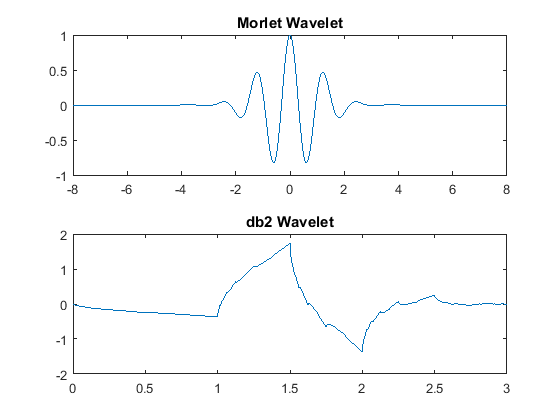
\includegraphics[]{morletvsdb2.png}
	\caption{A plot of the Morlet wavlet and the Daubechies order 2 wavelet produced by Matlab.}
	\label{fig:mvd}
\end{figure}

The discrete wavelet transform has many modifications to help it improve. Ebrahimi et al. \cite{ebrahimi_automatic_2008} used a wavelet packet tree (WPT), but there are many more such as the stationary wavelet transform (SWT), complex-valued wavelet transform (CWT), dual-tree complex wavelet transform (DTCWT), etc. Testing the differences in these modifications can be completed in a future study. 

This study used the multilevel discrete wavelet transform. Each level is the transform of the previous level. Each level is not as close to the originial wave as the previous level, but it greatly reduces the number of coefficients (a and b described above).



\section{\textbf{Categorization and Artificial Neural Networks}}

The purpose of this article is to classify REM sleep using the output of multilevel discrete wavelet transform. This paper was completed to use an artificial neural network (ANN), but there are some alternative classifcation algorithms. Alvarez et al. \cite{alvarez_usefulness_2017} listed the following algorithms, among others, in order of highest accuracy for sleep staging: ANN, support vector machine (SVM), hidden Markov models, and discriminant analysis. Lotte et al. \cite{lotte_review_2007} scored many algorithms for classification in EEG-based brain-computer interface including linear discriminant analysis, support vector machine (SVM), ANN multilayer perceptron, others ANNs, Bayes quadratic, hidden Markov model, k nearest neighbors, Mahalanobis distance, and combinations. Even though Lotte et al. \cite{lotte_review_2007} concluded that the SVM would be best for EEG-based brain-computer interface, they also stated neural networks are the most used category of classifier. Seeing that both Alvarez et al. and Lotte et al. put significance on SVMs and hidden Markov models, these two algorithms may be tested in the future.

There are many types of ANNs. Heaton \cite{heaton_artificial_2015} listed feedforward networks, deep belief networks, deep feedforward networks, and convolution networks as the best ANNs for classification. Other studies have had high accuracy with feed forward back propagation neural networks \cite{crasto_wavelet_2017} \cite{sinha_artificial_2008} and multilayer perceptron neural networks \cite{kurt_ann-based_2009} \cite{ventouras_sleep_2005}. All of these algorithms could be tested. This paper used a feed forward backward propagation neural network.

A neural network produces a non-linear decision boundary \cite{lotte_review_2007}. It is easy to understand a neural network when it is described from regression which produces a linear decision boundary. 

Linear regression is based on the equation of a line. The equation of a line is \(y = mx + b\). Given any set of x and y coordinates, there exist a line that minimizes the distance between the line and the coordinates \cite{lazyprogrammer.me_data_nodate-1}. In other words, there exist a red line that minimizes the sum of the lengths of the blue dashed lines in \ref{fig:linear}.

\begin{figure}[H]
	\centering
	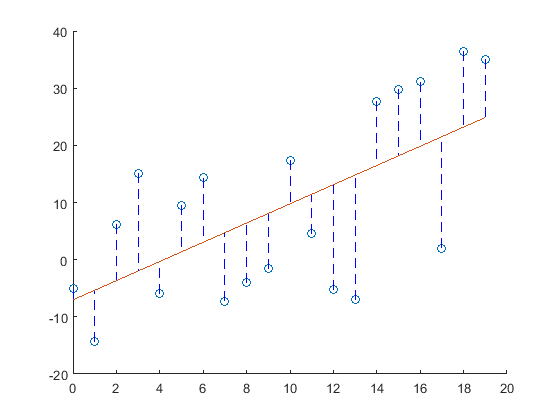
\includegraphics[]{linear.png}
	\caption{The plot of line that was produced via linear regression on a set of coordinates.}
	\label{fig:linear}
\end{figure}

If the coordinates of are represented by set \(x = [x_i] and y = [y_i] \) for i in range 1 to the number of points n and \(yhat = m*x + b\), where \(yhat = [yhat_i]\)  for i in range 1 to n, is the equation of a line with m and b unknown, then the sum of the distances between the line and the set is \( SUM_{i=1}^{n}|y_{i}-yhat_{i}| \) where \(|y-yhat|\) is the absolute value of \(y_{i}-yhat_{i}\). In linear regression, the the square of \(y_{i}-yhat_{i}\) is used instead of absolute value. This makes the equation for the sum of the distances from the line to the set of coordinates the least squares equation \cite{lazyprogrammer.me_data_nodate-1}

\begin{equation}
SUM_{i=1}^{n}(y_{i}-yhat_{i})^{2}.
\end{equation}

If yhat is replaced with the equation of a line, the least squares equation becomes the cost function for linear regression \cite{lazyprogrammer.me_data_nodate-1}

\begin{equation}
cost=C=SUM_{i=1}^{n}(y_{i}-(m*x_{i} + b))^{2}.
\end{equation}


In order to minimize this equation, the derivative with respect to m and b is taken and set equal to 0. This results in a system of two equations and two unknowns that can be solved. When x is multidimensional, the solution is still the same in the sense that the least squares equation is minimized. \cite{lazyprogrammer.me_data_nodate-1}

When there is not a solution to the multidimensional derivative of least squares, gradient descent can be used to find m and b. Gradient descent is stepping along the gradient of a function. Instead of solving for where the gradient equals zero by setting it to zero, gradient descent takes small steps towards gradient value zero until it reaches it. Mathematically, it looks like

\begin{equation}
w_{i+1} = w_{i} + \lambda * \nabla f(w_{i})
\end{equation}

where f is the least squares equation and lamda is the step size or the learning rate. The following image can help you visualize gradient descent. \cite{lazyprogrammer.me_data_nodate-1}
\begin{figure}[H]
	\centering
	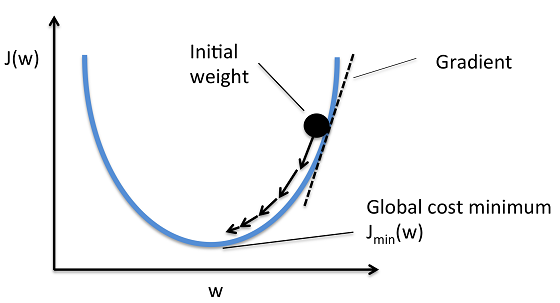
\includegraphics[]{gradDesc.png}
	\caption{Gradient Descent image from https://sebastianraschka.com/faq/docs/closed-form-vs-gd.html \cite{noauthor_machine_nodate}.}
	\label{fig:gradDesc}
\end{figure}

Let x and y be nodes. Let those nodes be represented by circles. The picture below is a picture of 1 sample of a function in 2 dimensions. Take note that this is a picture of one \(x_{i}\) and one \(y_{i}\) value or one sample. 
\begin{figure}[H]
	\centering
	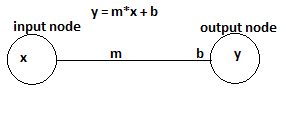
\includegraphics[]{lineNodes.png}
	\caption{Function in node picture.}
	\label{fig:lineNode}
\end{figure}

When this image is scaled up to multiple dimensions, it looks like.

\begin{figure}[H]
	\centering
	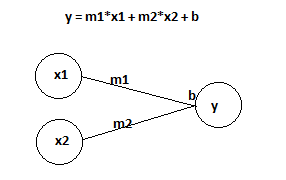
\includegraphics[]{mlineNodes.png}
	\caption{Function with multiple inputs in node picture.}
	\label{fig:mlineNode}
\end{figure}

In order to turn this picture from a linear regression picture to a logistic regression picture, the sigmoid function must be used. The sigmoid function returns a value between 0 and 1 always. \cite{lazyprogrammer.me_data_nodate-2}

\begin{equation}
s(x) = \frac{1}{1+e^{-x}}
\end{equation}

\begin{figure}[H]
	\centering
	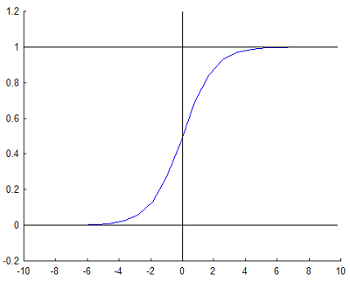
\includegraphics[]{sigmoid.png}
	\caption{Plot of the sigmoid function.}
	\label{fig:sigmoid}
\end{figure}

Once the sigmoid is applied, the nodes picture looks like the following. \cite{lazyprogrammer.me_data_nodate-2}

\begin{figure}[H]
	\centering
	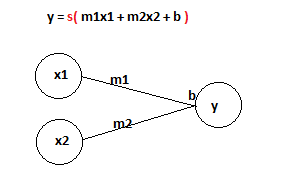
\includegraphics[]{sigNodes.png}
	\caption{Function with multiple inputs in sigmoid node picture.}
	\label{fig:sigNode}
\end{figure}

Now that this picture is logistic regression, the output is always between 0 and 1. Instead of using least squares as the cost function, the cross-entropy is used as the cost function. \cite{lazyprogrammer.me_data_nodate-2}

\begin{equation}
C=-\sum_{n=1}{N}y_{n}log(yhat_{n})+(1-y_{n})log(1-yhat_{n})
\end{equation}
y is the real solution, yhat is the solution from logistic regression, and  N is the number of samples. Just like with multiple linear regression, the derivative of the cross-entropy function C with respect to m and b is taken. When this derivative is set to 0, it can be solved in certain situations. In the situations where it can not be solved, the gradient descent method can be used to find the solution. \cite{lazyprogrammer.me_data_nodate-2}

The next step to reaching a neural network is to assume that there are multiple outputs per sample. The nodes picture becomes the following:
\begin{figure}[H]
	\centering
	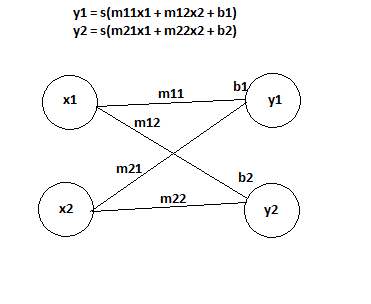
\includegraphics[]{ANNsigNodes.png}
	\caption{Function with multiple inputs and multiple outputs in a sigmoid node picture.}
	\label{fig:ANNsigNode}
\end{figure}

The final step in reaching a neural network is adding one more layer.

\begin{figure}[H]
	\centering
	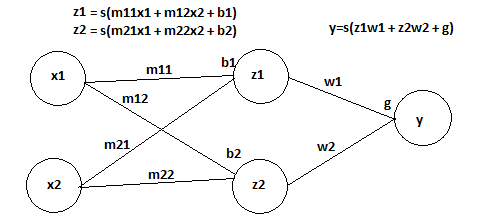
\includegraphics[]{ANNNodes.png}
	\caption{Function with multiple inputs and layers and a single in a sigmoid node picture.}
	\label{fig:ANNNode}
\end{figure}

Notice that the function for y, z1, and z2 is still sigmoid. For the middle layers, the sigmoid function can be replaced with 1 of many nonlinearity functions including hyperbolic tangent, linear, step, and rectified linear unites (ReLU) \cite{heaton_artificial_2015}. For the sigmoid function for y, there is a special case. While the function for y is sigmoid, the cost function can remain the cross-entropy function. When there are mutliple output nodes, there is a special function called the softmax function which should be used. \cite{lazyprogrammer.me_data_nodate}

\begin{equation}
softmax=sf=\frac{a_{k}}{\sum_{j=1}^{K}a_{j}}
\end{equation}
where K is the number of nodes in the layer before y and
\begin{equation}
a_{k} = \sum_{i=1}^{K}w_{ik}*z_{i}
\end{equation}
where \(z_{i}\) is the ith node of the previous layer. \cite{lazyprogrammer.me_data_nodate} The nodes picture become the following: 

\begin{figure}[H]
	\centering
	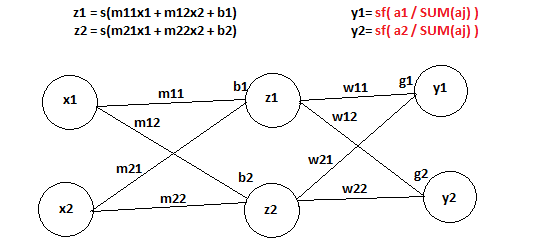
\includegraphics[]{mANNNodes.png}
	\caption{Function with multiple inputs, layers, and outputs in a ANN node picture.}
	\label{fig:mANNNode}
\end{figure}

When the softmax function is used, the cost function becomes the multiclass log likelihood (ll) function 
\begin{equation}
C =ll = \sum_{n=1}^{N} \sum_{k=1}^{K} y_{k}^{n}log(yhat_{k}^{n})
\end{equation}
where N is the number of samples and K is the number of outputs. Once again, the derivative of this function is taken. The variables w, g, m, and b, or the weights and biases, are solved for using gradient descent. This is the feed forward backward propagation artificial neural network used for this study. \cite{lazyprogrammer.me_data_nodate}


\chapter{\textbf{METHODS AND RESULTS}}

\section{\textbf{Methods}}
This study used the "Sleep Recording and Hypnograms in European Data Format (EDF)" data set or "The Sleep-EDF Database [Expanded]" from physionet.org \cite{noauthor_sleep-edf_nodate}. The portion of the database used is from a study on healthy patients from 1987-1991. There are 20 patients avaialable. There are 10 males and 10 females ranging from age 25-34 years old \cite{noauthor_sleep-edf_nodate}. 

Each patient had two relevant files: a polysomnogram (PSG) recording in EDF format and a hypnogram of annotations in EDF+ \cite{noauthor_sleep-edf_nodate}. EDF is a standard format for exchanging EEG recordings \cite{noauthor_european_nodate}. EDF+ has all the capabilities of EDF and the ability to contain annotations \cite{noauthor_european_nodate}. The PSG recording included an EEG from Fpz-Cz and Pz-Oz electrode locations, an EOG (horizontal), a submental chine EMG, an event marker, an oral-nasal respiration, and rectal body temperature. The hypnogram is an annotation of sleep patterns. The annotations included W for wakefulness, R for REM, 1 for stage 1, 2 for stage 2, 3 for stage 3, 4 for stage 4, M for movement time and ? for not scored. Once the first annotation was reached, the rest of the annotations were 30 seconds apart creating the 30 second epochs.

Special software is required to read the EDF and EDF+ files. EDFbrowser is a free EDF and EDF+ reader that can export the contents to a text file. All the contents of the PSG and hypnogram file were exported to a text file with the option to have time in seconds from the first recording.

The PSG and hypnogram text files were imported into a custom python 3 script. The python 3 script, epochs.py, used the pywavelets package to complete a wavelet decomposition of any suggested level. The output file contains the annotation and decomposition of each epoch per line unless the annotation is for movement time or not scored. Movement time and not scored epochs are skipped in a majority of the tests. The count of each annotation per file is printed to standard out.

The EEG has a recording every 10 milliseconds. There are 3000 recordings per epoch. This implies that the maximum decomposition level is 8. Each decomposition level produced a different number of coefficients listed in table \ref{tab:coeff}.

\begin{table}[H]
	{\hspace{0cm}
		\begin{tabular}{|c|c|c|c|c|c|}
			\hline \\ [-1.5ex]
			\textbf{Level} & \textbf{\# of Coefficients} \\
			\hline \\ [-1.5ex]
			8&14 \\
			\hline \\ [-1.5ex]
			7&26 \\
			\hline \\ [-1.5ex]
			6&49 \\
			\hline \\ [-1.5ex]
			5&96 \\
			\hline \\ [-1.5ex]
			4&190 \\
			\hline \\ [-1.5ex]
			3&377 \\
			\hline \\ [-1.5ex]
			2&752 \\
			\hline \\ [-1.5ex]
			1&1501 \\
			\hline
		\end{tabular}
	} 
	\caption{The number of coefficients produced for a 30 second epoch at each available level of decomposition.}
	\label{tab:coeff}
\end{table}

The python 3 script for the feed forward backward propogation artificial neural network, softANN.py, accepted the output of epochs.py as input. The input file is put into a special format for the input to the neural network. The real value of the output of the neural network is y = [1,0] if the annotation is R and [0,1] if the annotation is not REM. The input to the neural network consist of the coefficients from 3 epochs: the prior epoch, the current epoch, and the post epoch. If the current epoch is the first epoch in the file then all the coefficients to the prior epoch are set to zero. If the current epoch is the last epoch in the file then all the coefficients of the post epoch are set to 0. 

softANN.py does the training and prediction testing of the artificial neural network. The outputs for training are 4 CSV files and current statistics to standard out at specified intervals. The 4 CSV files are the weights and biases between the input and hidden layers and the hidden and output layers. The current statistics include the cost and the accuracy of the weights and biases. The stopping condition was split between 100\% accuracy and cost less than \(10e^{-1}\). The output for prediction testing includes the accuracy, sensitivity, and specificity \cite{baratloo_part_2015}.

\section{\textbf{Results}}

Because each patient has 2 nights of recordings, there are 40 nights available from the sleep EDF database. Of the 40 nights available, 24 were used. Excluding movement time and not scored, there were an average of 1589 epochs per night. Of those epochs, 89\% were not REM and 10\% were REM.

Using one of the nights, some preliminary test were run on the softANN.py to determine the optimal wavelet decomposition level, the optimal number of hidden nodes, and the optimal learning rate. It appears any level is capable of achieving 100\% accuracy on the test night. Lower levels achieve 100\% accuracy while reducing the Cost more than higher levels. The difference in time to 100\% between levels is negligible. 10e-5 is the optimal learning rate for all levels. It was found that learning rates 10e-3 and larger caused an overflow. Crasto et al. \cite{crasto_wavelet_2017} used principal component analysis to reduce the number of coefficients from approx 3000 to 400. These wavelet levels can reduce the number of components to 14, but level 3 reduces the number of coefficients to 377 which is closest to 400. Since 3 epochs are used, there are 1131 input nodes with 3 levels of decomposition. Various numbers of hidden nodes were tested, but the results were not stored. The number of hidden nodes were set to half the number of input nodes, equal the number of input nodes, and one and a half the number of input nodes with no difference noticed. The test for training and predictions all used the same number of hidden nodes as input nodes. 

The training data sets were all used 1, 2, or 4 nights of data. Of the 8 trainings, 1 was stopped by the user, 1 resulted in overflow, and 1 had the weights lost as a result of a copying error. The training stopped by the user was stopped after 3 days. No other training took longer than 12 hours. All of the training was stopped in the program when the accuracy of the current data set reached 100\% except 1 which was stopped after the cost reached 10e-1. The results of the trainings are listed in table \ref{tab:train}. Each training set was given an id based on the level of decomposition and the number of iterations of training. The level of decomposition is the first number and the number of iterations is the second number in the id.

\begin{table}[H]
	{\hspace{0cm}
		\begin{tabular}{|c|p{2cm}|c|c|c|c|c|c|}
		\hline \\ [-1.5ex]
		\textbf{ID}      & \textbf{DATA}                          & \textbf{Learning Rate} & \textbf{Result}   & \textbf{Final Cost}  & \textbf{STOP}                \\
		\hline \\ [-1.5ex]
		3.15000 & Patient 001 + 031 + 101 + 161 & 10e-5         & Copy Error & -4.45          & Accuracy = 100\\
		\hline \\ [-1.5ex]
		3.3000  & Patient 001                   & 10e-5         & Complete & -16        & Accuracy = 100\\
		\hline \\ [-1.5ex]
		3.36000 & Patient 001                   & 10e-5         & Complete & -0.99      & Cost \textless 10e-1  \\
		\hline \\ [-1.5ex]
		3.6000  & Patient 001 -\textgreater101  & 10e-5         & Complete & -26.9      & Accuracy = 100 \\
		\hline \\ [-1.5ex]
		3.85000 & Patient 001 + 101             & 10e-5         & Complete & -16.16     & Accuracy = 100 \\
		\hline \\ [-1.5ex]
		2.5500  & Patient 001 + 101             & 10e-5         & Complete & -6.07      & Accuracy = 100\\
		\hline \\ [-1.5ex]
		2.?1    & Paitent 001+031+101+161       & 10e-5         & OVERFLOW &            & Accuracy = 100 \\
		\hline \\ [-1.5ex]
		2.?2    & Paitent 001+031+101+161       & 10e-7         & Stopped  &            & Accuracy = 100 \\    
		\hline
	\end{tabular}
} 
\caption{The results of the training sessions.}
\label{tab:train}
\end{table}

Each training session produced weights and biases that were used to make test predictions. the test predictions were completed with all of the remaining nights. The average accuracy, sensitivity, and specificity are listed in table \ref{tab:pred}.

\begin{table}[H]
	{\hspace{0cm}
		\begin{tabular}{|c|c|c|c|}
			\hline \\ [-1.5ex]
			ID      & Accuracy & Sensitivity & Specificity \\
			\hline \\ [-1.5ex]
			3.15000 & 89.98\%  & 38.07\%     & 96.38\%     \\
			\hline \\ [-1.5ex]
			3.3000  & 79.67\%  & 36.01\%     & 89.82\%     \\
			\hline \\ [-1.5ex]
			3.36000 & 84.40\%  & 29.89\%     & 91.83\%     \\
			\hline \\ [-1.5ex]
			3.6000  & 85.82\%  & 17.54\%     & 93.30\%     \\
			\hline \\ [-1.5ex]
			3.85000 & 81.12\%  & 42.79\%     & 88.20\%     \\
			\hline \\ [-1.5ex]
			2.5500  & 83.49\%  & 39.14\%     & 88.63\%  \\   
			\hline
		\end{tabular}
	} 
	\caption{The results of the training sessions.}
	\label{tab:pred}
\end{table}


\chapter{\textbf{CONCLUSIONS AND FUTURE}}

\section{\textbf{Conclusions}}

There are many factors left formerly untested: Over-fitting as a stopping condition in training, the number of nodes in the hidden layers, the number of hidden layers,  more than 2 nights as input, level 2 decomposition, etc. 

The best result is that the ability to pick REM sleep is not good. The percentage of correctly chosen REM was less than 50\% a majority of the time. Sensitivity increases when the number of nights included in the input increased. There are not enough test to know if lowering the decomposition level had an effect. 

A positive result is the specificity which was consistently near or above 90\%. 

The results support the idea that all sleep stages besides REM are easier to find in a single channel EEG. 

\section{\textbf{Future Work}}

In future studies, every aspect of this study could be changed to improve necessary results. The choice of EEG channel. The choice of sleep channel. The choice of sleep stage could be changed. The choice of epoch size could be changed. Of time-frequency techniques, the wavelet transform is the best choice, but the modification of wavelet transform should be changed to possibly a continuous wavelet transform or a new modification of the discrete wavelet transform. The support vector machine, multilayer perceptron, convolution neural networks, deep feed forward neural networks, and the hidden Markov model should all be tested for classification. 

This study was limited to a choice between two sleep channels. For at home studies, there are different devices that use different channels. One device uses a two electrodes around the Fpz electrode position. This position is basically on the forehead of a person and would be one of the easiest positions to locate for an untrained person. 

The goal of this paper is to support an at home sleep study. A sleep study needs to be able to detect all stages, but it is very important for a sleep study to identify sleep from wakefulness. If REM can not be identified, all stages can not be identified with a single channel EEG.

The epoch was originally defined based on the ease of use. The complication of paper size and time required for an analysis can be eliminated in choice of epoch size. A training dataset may be difficult to find for a small epoch size, but each individual wave can be classified based on the definitions provided by the AASM. This could result in epochs being scored literally by which waves make up the majority of the epoch.

Time-frequency analysis has many new modifications for discrete wavelet transforms. These modifications should be tested for improvements to the current discrete wavelet transforms. Also, the continuous wavelet transform (CWT)can contain more detail than the discrete wavelet transform (DWT). The CWT should be test against the new modifications of the DWT.

	
\bibliographystyle{myplain}
\clearpage
\markboth{}{}
\addcontentsline{toc}{chapter}{BIBLIOGRAPHY}
\bibliography{EEGApneaAll}
%references}


\end{document}